\chapter{實證分析}
\label{c:implement}
本研究使用「鉅亨網台股新聞」資料庫資料進行研究。利用自然語言處理方法正規化新聞文本資料後,利用創新 Ing and Lai (2011) 所提出之OGA模型之OGA Predict方法以及創新Chen, Dai, Ing, Lai所改量Temlyakov (2015)所提出之 CGA 模型之CGA Predict方法量化個股新聞情緒分數,建立個股投資組合並計算隔日報酬。

實證分析中,本研究利用迴歸係數之大小作為情緒排名之依據,正係數越大代表此情緒字詞對於股票報酬越有正面影響,反之亦然。該研究貢獻為,投資人是否會因為個股新聞之用詞好壞而影響投資決定,並比較股票價格與新聞發佈時間之領先滯後關係,投資人是否可掌握未發布之新聞消息。好讓我們可以理解到,新聞文章是如何影響到個股的報酬與投資績效的。
\section{資料來源與敘述統計}
本研究使用「鉅亨網台股新聞」資料進行研究,資料區間涵蓋2010年1月1日至2021年1月11日。$\ldots$
\begin{table}[H]
\begin{center}
\begin{tabular}[c]{lm{5cm}<{\centering}m{5cm}<{\centering}}
\toprule
& 剩餘樣本數 & 移除樣本數\\
\hline
鉅亨網新聞總數 & 1,238,618 & - \\
移除未標記股票之新聞 & 780,460 & 458,158 \\
移除標記多支股票新聞 & 667,399 & 113,061 \\
移除重複新聞 & 667,394 & 5 \\
移除公告類新聞 & 70196 & 587198\\
\bottomrule
\end{tabular}
\end{center}
\caption{鉅亨網台股新聞資料統計}
\label{Tab 4.1}
\end{table}

\newpage

\begin{figure}[htbp]
\centering
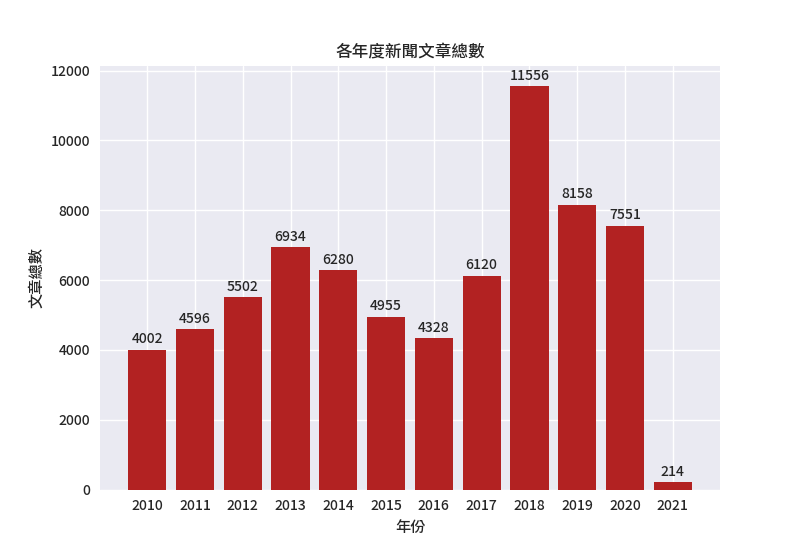
\includegraphics[width=0.7\textwidth]{/Users/chengchanglei/Desktop/CCL/Paper Code/3. Data Description/total_article_num_year.png}
\caption{每年發佈之新聞文章總數時間序列圖}
\end{figure}
圖4.1顯示了2010年1月1號至2021年1月31號之鉅亨網台股新聞資料庫在樣本內所使用之每年新聞文章總數,在樣本中每年平均有6,445篇新聞文章。觀察圖4.1可發現,近年來之新聞數量大於往年之發布新聞數量,顯示近年來非結構化數據之增長。

\begin{figure}[H]
\centering
\includegraphics[width=1.09\textwidth]{/Users/chengchanglei/Desktop/CCL/Paper Code/3. Data Description/output.png}
\caption{新聞文章平均(每日/每半小時)}
\end{figure}
圖4.2上半部繪製了樣本內每天平均發佈之新聞文章數量,由此圖可以看見二月所發布之新聞文章數相較於其他月份來得少,推測可能因為受新年假期以及閏月之影響。下半部則依每半小時為單位,繪製了每半小時平均發佈之新聞數量,從該圖可發現台股開盤時以及開盤後至晚間發布新聞頻率較為頻繁。

\clearpage

\section{資料預處理及統計分析流程}
本節介紹新聞文本資料預處理。中文文本在進行斷詞時,不像英文文本可以透過單詞間的空格直接將新聞文本轉換為單詞儲存即可完成斷詞過程,由於中文文本皆為連續的單詞或詞彙,尚無一套有效之標準流程針對中文文本進行自然語言處理任務的前置作業。

目前中文之自然語言處理以對岸所發明之簡體中文斷詞工具「結巴分詞」 (Jieba) 以及台灣中研院資訊所、語言所成立的語言研究小組針對繁體中文所開發的「中文自然語言處理的資源及研究環境」(Chinese Knowledge and Information Processing, CKIP)。使用者可以利用這些系統對中文文本進行自然語言處理作業,包含斷詞 (Tokenization)、詞性標記 (Part-of-Speech)等自然語言任務。

接著本節將詳細的介紹本研究如何利用自然語言處理之結果對新聞文本進行資料預處理。以下步驟為自然語言處理之正規化(Normalization)流程。第一步將專有名詞移除(如:人名與公司名稱等),由於公司名稱為對應個股股價報酬之標記方式,並假設該篇個股新聞之內容將影響單一個股報酬,因此公司名稱在本次的實驗設計中設定為投資人選擇的個股標籤而非影響股價報酬之詞彙,所以將公司名稱當作專有名詞將其刪除;第二步移除數字、標點符號、特殊符號等非中文詞彙;第三步移除中文停止詞或修飾詞(如:「是」、「的」、「和」等)。最後將所收集到之新聞文章以單詞列表的形式儲存於資料庫中以利後續分析使用。
\subsection{自然語言處理}
本研究在中文斷詞上採用中研院針對『繁體中文』訓練一系列的 Transformer 模型,包含 ALBERT、BERT、GPT2。除了訓練語言模型外, 該系統亦針對各個自然語言任務上訓練了對應的模型(包含斷詞、詞性標記、實體辨識)以資料集中其中一篇文檔做範例如下:
\\[0.6ex]
\begin{tcolorbox}

{\textcolor{blue}{記憶體封測廠力成 (6239-TW) 今(5)日傳出發生氣爆,對此力成回應,僅是3C廠區內發生小事故,但未造成人員傷亡,也沒有對生產或營運造成任何影響。}}
\end{tcolorbox}

\newpage

CKIP斷詞後結果整理如下:
\begin{table}[H]
\begin{center}
\begin{tabular}[c]{l|m{0.3cm}<{\centering}m{0.3cm}<{\centering}m{0.3cm}<{\centering}m{0.5cm}<{\centering}m{0.5cm}<{\centering}m{0.5cm}<{\centering}m{0.3cm}<{\centering}m{0.5cm}<{\centering}m{0.3cm}<{\centering}m{0.3cm}<{\centering}m{0.3cm}<{\centering}m{0.3cm}<{\centering}m{0.5cm}<{\centering}m{0.3cm}<{\centering}m{0.3cm}<{\centering}m{0.5cm}<{\centering}m{0.2cm}<{\centering}m{0.3cm}<{\centering}}
\toprule
單詞& 記憶體 & 封測廠 & 力成 & ( & 6239-TW & ) & 今 & (5) & 日 & 傳出 & 發生 & 氣爆 & , & $\cdots$ & 造成 & 任何 & 影響 & 。 \\
\hline
詞性 & Na & Nb & Nb & Pun. & Neu & Pun. & Nd & Neu & Nd & VC &  VJ & VH & Pun. & $\cdots$ & VK & Vega & Na & Pun. \\
\hline
實體辨識 &  &  & 人物 &  &  & & 日期 & 日期 & 日期 &  &  &  &  &  &  &  &  &  \\
\bottomrule
\end{tabular}
\end{center}
\caption{CKIP斷詞結果}
\label{Tab 4.2}
\end{table}
上述顯示了透過 CKIP 針對繁體中文進行自然語言處理作業之流程,顯示了欲分析之例句以及進行斷詞、詞性標記及實體辨識三種不同之自然語言任務之結果。目的在於辨識出例句中,具有特定意義之單詞,例如,7 月 22 日(日期)、程小明 (人物)、新北市(地點)等具有通俗定義之單詞,而透過實體辨識則可以辨識出目標文本中之專有名詞、時間日期等無情緒詞彙。
\subsection{正規化}
此節詳述了針對繁體中文進行自然語言處理之正規化之過程與結果。正規化 (Normalization) 主要之步驟包含移除『專有名詞』、『日期』等字詞、移除數字、標點符號、特殊符號等非中文詞彙、移除中文停止詞或修飾詞  (e.g., 『和』, 『的』, 『是』, 『也』等),正規化範例如下表格所示:
\begin{table}[H]
\begin{center}
\begin{tabular}[c]{l|m{0.3cm}<{\centering}m{0.3cm}<{\centering}m{0.3cm}<{\centering}m{0.5cm}<{\centering}m{0.5cm}<{\centering}m{0.5cm}<{\centering}m{0.3cm}<{\centering}m{0.5cm}<{\centering}m{0.3cm}<{\centering}m{0.3cm}<{\centering}m{0.3cm}<{\centering}m{0.3cm}<{\centering}m{0.5cm}<{\centering}m{0.3cm}<{\centering}m{0.5cm}<{\centering}m{0.5cm}<{\centering}m{0.2cm}<{\centering}m{0.3cm}<{\centering}m{0.3cm}<{\centering}m{0.3cm}<{\centering}m{0.3cm}<{\centering}}
\toprule
單詞 & 記憶體 & 封測廠 & \textcolor{purple}{力成} & \textcolor{teal}{(} & \textcolor{teal}{6239-TW} & \textcolor{teal}{)} & \textcolor{purple}{今} & \textcolor{purple}{(5)} & \textcolor{purple}{日} & 傳出 & 發生 & 氣爆 & \textcolor{teal}{,} & \textcolor{cyan}{對} & \textcolor{cyan}{此} & \textcolor{purple}{力成} & 回應 \\
\hline
詞性 & Na & Nc & Nb & Pun. & Neu & Pun. & Nd & Neu & Nd & VC &  VJ & VH & Pun. & P & Nep & Nb & VC \\
\hline
實體辨識 &  &  & 人物 &  &  & & 日期 & 日期 & 日期 &  &  &  &  & \\
\bottomrule
\end{tabular}
\end{center}
\caption{CKIP正規化結果}
\label{Tab 4.3}
\end{table}

\begin{table}[H]
\begin{center}
\begin{tabular}[c]{l|m{0.5cm}<{\centering}m{0.3cm}<{\centering}m{0.5cm}<{\centering}m{0.5cm}<{\centering}m{0.3cm}<{\centering}m{0.5cm}<{\centering}m{0.3cm}<{\centering}m{0.5cm}<{\centering}m{0.5cm}<{\centering}m{0.5cm}<{\centering}m{0.3cm}<{\centering}m{0.3cm}<{\centering}m{0.5cm}<{\centering}m{0.3cm}<{\centering}m{0.5cm}<{\centering}m{0.5cm}<{\centering}m{0.2cm}<{\centering}m{0.3cm}<{\centering}m{0.3cm}<{\centering}m{0.3cm}<{\centering}m{0.3cm}<{\centering}}
\toprule
單詞 & \textcolor{teal}{,} & \textcolor{cyan}{僅} & \textcolor{cyan}{是} & \textcolor{teal}{3C} & 廠區 & \textcolor{cyan}{內} & 發生 & \textcolor{cyan}{小} & 事故 & \textcolor{cyan}{但} & \textcolor{cyan}{未} & 造成 & 人員 & 傷亡 & \textcolor{teal}{,} & \textcolor{cyan}{也} & 沒有 \\
\hline
詞性 & Pun. & Da & SHI & FW & Nc & P & VC & VH & Na & Cbb & D & VK & Na & VH & Pun. & D & D \\
\hline
實體辨識 &  &  &  &  &  & &  &  &  &  &  &  &  & \\
\bottomrule
\end{tabular}
\end{center}
\caption{CKIP正規化結果}
\label{Tab 4.4}
\end{table}

\begin{table}[H]
\begin{center}
\begin{tabular}[c]{l|m{0.5cm}<{\centering}m{0.5cm}<{\centering}m{0.5cm}<{\centering}m{0.5cm}<{\centering}m{0.5cm}<{\centering}m{0.7cm}<{\centering}m{0.5cm}<{\centering}m{0.5cm}<{\centering}}
\toprule
單詞 & \textcolor{cyan}{對} & 生產 & \textcolor{cyan}{或} & 營運 & 造成 & 任何 & 影響 & \textcolor{teal}{。} \\
\hline
詞性 & P & VC & Caa & VA & VK & Neqa & Na & Pun. \\
 \\
\hline
實體辨識 &  &  &  &  &  &  &  & \\
\bottomrule
\end{tabular}
\end{center}
\caption{CKIP正規化結果}
\label{Tab 4.5}
\end{table}

第一步移除專有名詞(上表標註之紅色單詞),此步驟根據實體辨識結果,移除 CKIP 可辨識之特定意義詞彙(e.g., 組織:力成; 人名:張忠謀; 日期: 5 日、上午 9 時; 地名: 台北市、臺灣, etc.),透過該系統可移除文本中大量專有名詞,解決了中文自然語言處理一大難處。

第二步為移除數字、標點符號及特殊符號等非中文詞彙(上表標註為綠色之單詞),此步驟利用詞性標記及特殊符號字典交互進行,移除詞性被標記為「數 字」、「標點符號」、「英文」亦或該單詞存於特殊符號字典中之詞彙。

第三步為移除中文停止詞或修飾詞(上表標註為藍色之單詞),中文停止詞與修飾詞(e.g.「和」、 「的」、「是」、「也」etc.)在中文上無特殊意義,保留此類單詞易造成模 型有過多噪音。至此,可完成正規化作業。

\newpage

\subsection{資料預處理與統計分析流程}

\begin{figure}[htbp]
\centering
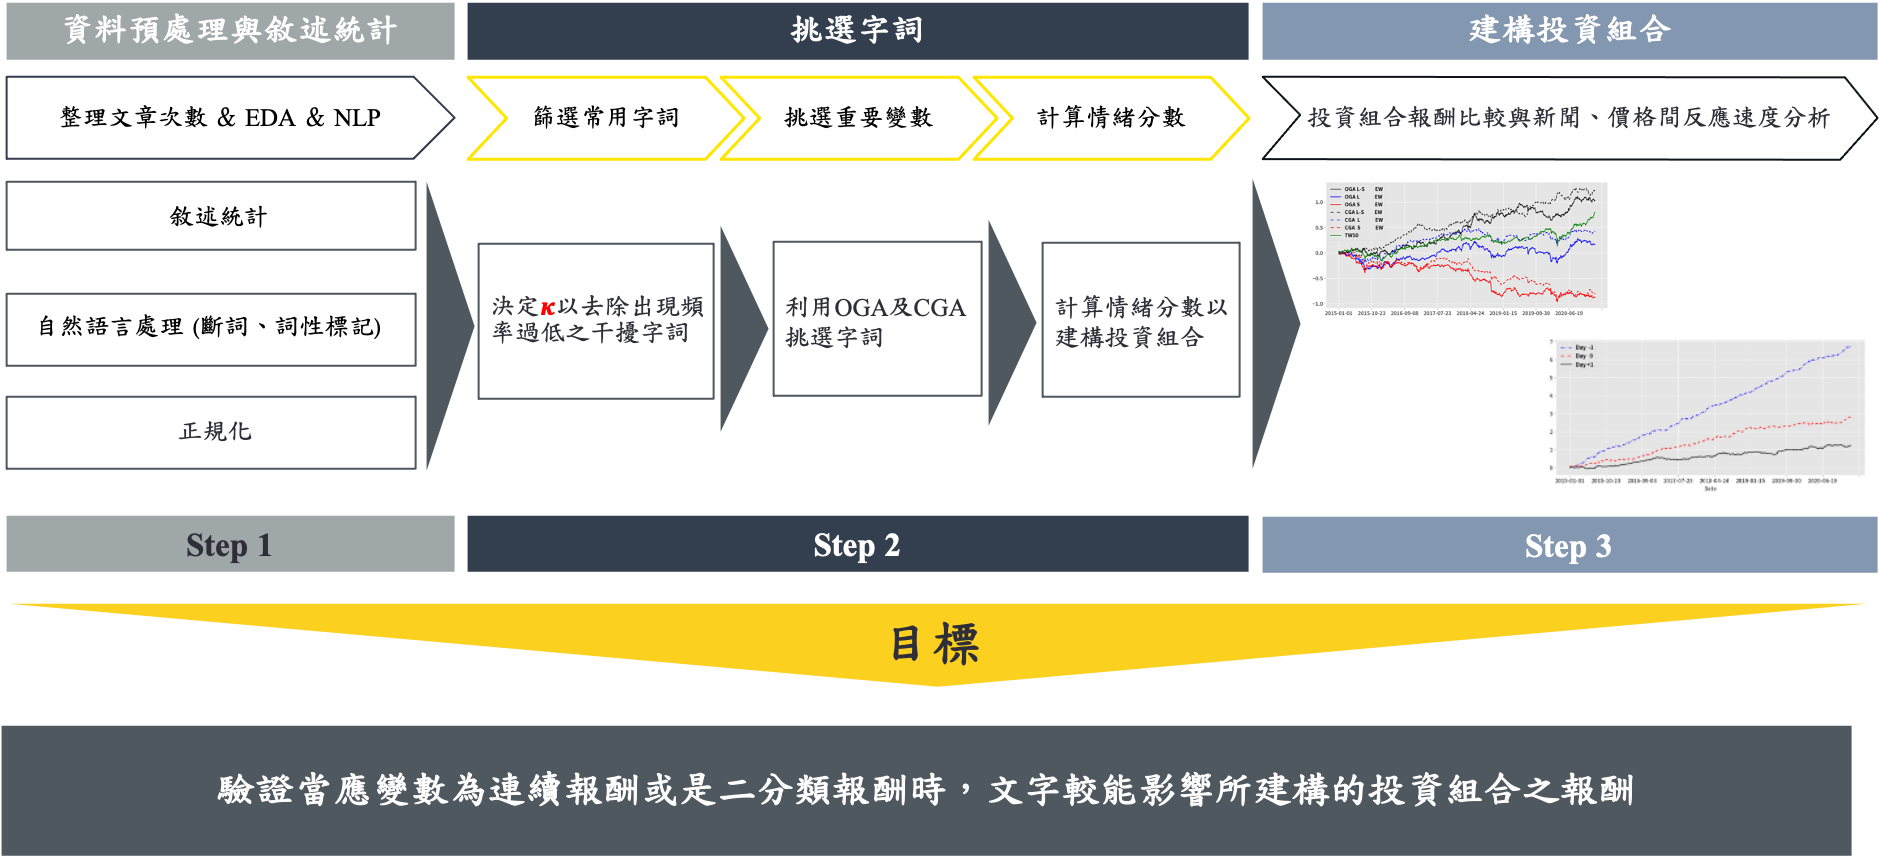
\includegraphics[width=1.1\textwidth]{images/流程圖.png}
\caption{統計分析流程圖}
\end{figure}



\section{實證結果}
本節將建構台股新聞情緒模型,以計算每日情緒分數並建構交易策略及投資組合,進而實證當應變數報酬為線性假設或者是非線性假設時,何者能有較好的超額報酬。以及驗證在散戶為主的台灣市場中之間隔延遲關係,並透過在不同條件之下(市值、波動度)探討台灣股市之新聞反應速度。
\subsection{預測股票報酬}
此小節將詳述如何訓練模型並估算每日新聞情緒分數。以五年為一個滾動(rolling)週期,樣本內前五年用於訓練,同時根據滾動週期,使用樣本週期後一年進行樣本外測試(ex:第一個rolling為2010年至2014年,並利用2015年進行測試)。在每次測試年份結束後,將整個訓練週期向後滾動一年並重新訓練模型,直到用盡所有樣本資料為止。完成模型訓練及情緒分數估算後,透過估算出之情緒分數建構隔日投資組合,參考 Ke, Kelly, and Xiu (2019) 將台灣時間 09:00 a.m. 至隔日 09:00 a.m. 時間區間定義為一天,並且將 Day 0所蒐集之新聞文章計算情緒分數後,用以建構隔日投資組合。當中將台灣時間 08:30 a.m. 至 09:00 a.m.所發佈之新聞移除不用於測試集交易,其目的在於希望模型用於測試集交易時能更加的貼近真實情況,例如基金公司於開盤前便已針對前一天所發佈之新聞決定當日部位變動,若使用過於接近開盤時所發佈之新聞,可能造成基金公司或投資人沒有充足的時間計算部位以因應在流動性高峰期間進行交易。

本研究針對Day 0所發佈之個股新聞,將於Day 1開盤時建構投資組合部位,並於隔日開盤時將所持有的部位平倉,稱為隔日報酬投資組合。由上述做法,每天開盤都會建構新的投資組合,並持有部位1天,使用此種策略原因主要有以下兩點:第一,於收盤過夜期間所發佈之新聞,最可能於隔日市場開放的早期影響股票價格,因為該段時間是大多數交易者進入市場的時間。第二,除了從事高頻交易基金的公司之外,其餘基金公司之風險控管及資金限制等因素,不太可能根據盤中才出現的新聞消息而不斷地調整部位,因此透過衡量新聞對於隔日報酬的影響,能有效地得知前一天所發佈之新聞是否能影響投資人決策而影響股價。

\begin{figure}[htbp]
\centering
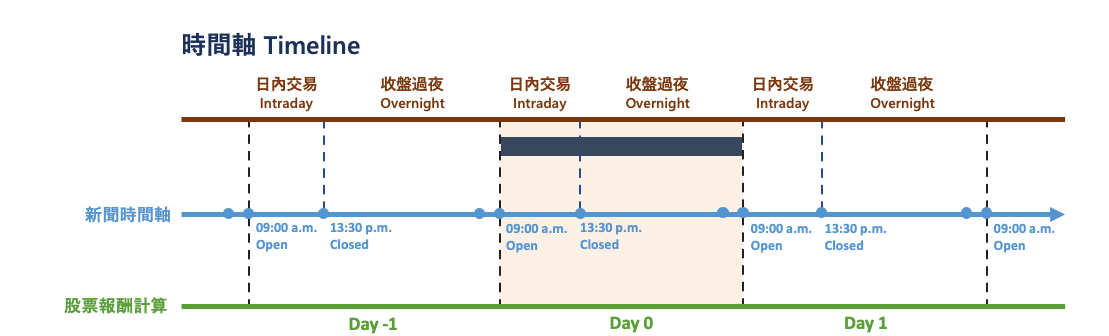
\includegraphics[width=1.1\textwidth]{images/times.png}
\caption{交易時間軸}
\end{figure}


\subsection{字詞挑選結果}
\begin{figure}[htbp]
\centering

\includegraphics[width=1.1\textwidth]{images/OGA result.png}
\caption{OGA 字詞挑選結果}
\end{figure}

\begin{figure}[htbp]
\centering

\includegraphics[width=1.1\textwidth]{images/CGA result.png}
\caption{CGA 字詞挑選結果}
\end{figure}
圖4.5與圖4.6分別為OGA以及CGA所挑選出來與報酬最相關之正面與負面情感詞,由於訓練週期會不斷改變,且會重新估算情緒分數,因此分析過程中,情感詞列表也會不斷地改變。如前述所說本研究共有兩種參數$\kappa$ 與 $k$,而本研究參考Fan, et al.(2021)之實證流程,由70\%至90\%且每2\%為一間隔挑選$\kappa$;而$k$則由100至500進行實證分析。我們找出報酬最高之參數為代表進行後續之實證分析。上述兩圖以投資組合中報酬最高為代表所挑出之情感詞。


\subsection{投資組合報酬比較}
本研究藉由情緒分數模型建構一日交易策略,我們蒐集第T天所發佈之新聞文章,並估算第T天所有新聞文章之情緒分數,並將所估算之情緒分數於第T+1天開盤時建構投資組合。於投資組合的多頭部位買進情緒分數最高的5篇新聞所對應之五檔公司股票,於投資組合的空頭部位則賣出情緒分數最低的5篇新聞所對應之五檔公司股票。除此之外,也考慮等權重(Equal-Weight, EW)及市值權重(Value-Weight, VW)兩種不同買賣方式之投資組合績效,等權重將所持有資金「等比例」配置於所持有之五檔作多股票及五檔作空股票;市值權重則將所持有資金依「市值」配置於所持有之五檔作多股票及五檔作空股票。在評估績效方面,我們考慮了等權重多空部位(EW L-S)、等權重多頭部位 (EW L)、等權重空頭部位(EW S)、市值權重多空部位(VW L-S)、市值權重多頭部 位(VW L)、市值權重空頭部位(VW S),總共六種不同的配對投資組合策略,將相同策略進行比較(多空策略與多空策略比較、多頭策略與多頭策略比較、空頭策略與空頭策略比較),並將以上投資組合與買進並持有(Buy and Hold)臺灣50相比較,最後透過評估投資組合績效確認基於情緒分數模型所建構之投資組合策略是否有顯著超額報酬。

\newpage

\begin{figure}[htbp]
\centering
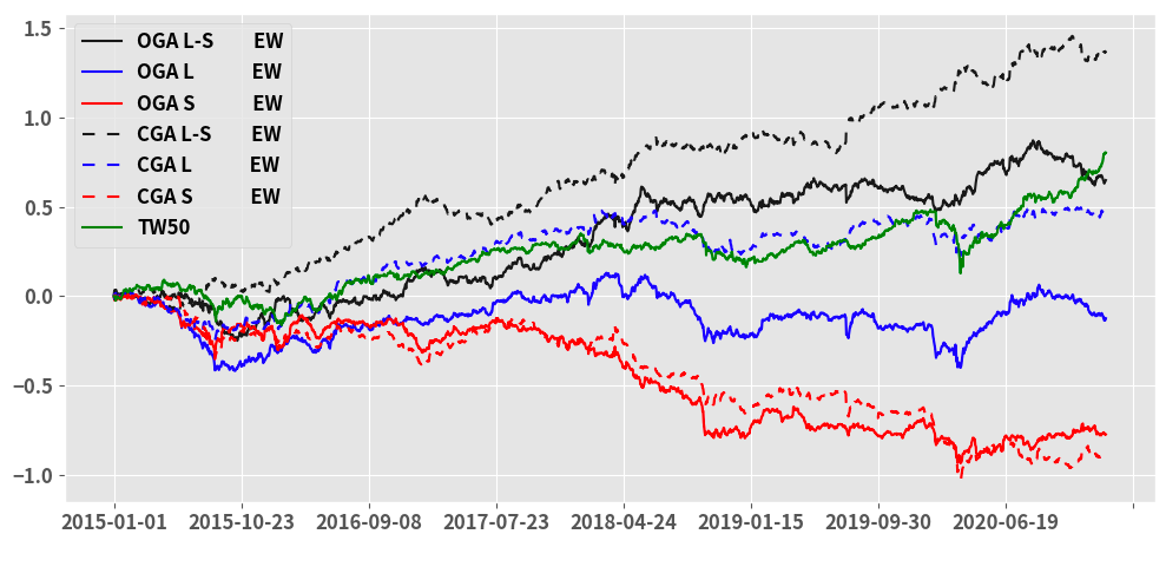
\includegraphics[width=1.1\textwidth]{images/OGA vs CGA.png}
\caption{OGA v.s CGA}
\end{figure}

於圖4.7繪製了利用情緒分數所建構之投資組合其「樣本外」累積對數報酬。黑線、藍線及紅線分別表示多空部位(Long-Short)、多頭部位(Long)及空頭部位(Short)之投資組合。實線及虛線則分別表示OGA及CGA兩種不同之模型假設之投資組合績效。綠色實線表示買進並持有臺灣50 (TW50)之報酬。而以夏普值(Sharpe Ratio)以及平均報酬(Average Return)來看,不管在多空策略、多頭策略或者是空頭策略上,CGA Predict皆比OGA Predict來得好,所以在接下來的分析之中皆以CGA所建構之情緒分數模型進行以下的實證分析。
\begin{table}[H]
\begin{center}
\begin{tabular}[c]{m{5cm}<{\centering}m{5cm}<{\centering}m{5cm}<{\centering}}
\toprule
 & 夏普值  & 平均報酬 \\
交易策略 & Sharpe Ratio & Average Return \\
\hline
OGA EW L-S & 0.52 & 3.33 \\
OGA EW L & -0.11 & -0.64 \\
OGA EW S & 0.73 & 3.97 \\
CGA EW L-S & 1.18 & 6.97 \\
CGA EW L & 0.45 & 2.36 \\
CGA EW S & 0.83 & 4.61 \\
TW 50    & 0.74 & 4.12 \\
\bottomrule
\end{tabular}
\end{center}
\caption{新聞情緒分數投資組合表現}
\label{Tab 4.6}
\end{table}

\newpage

\begin{figure}[htbp]
\centering
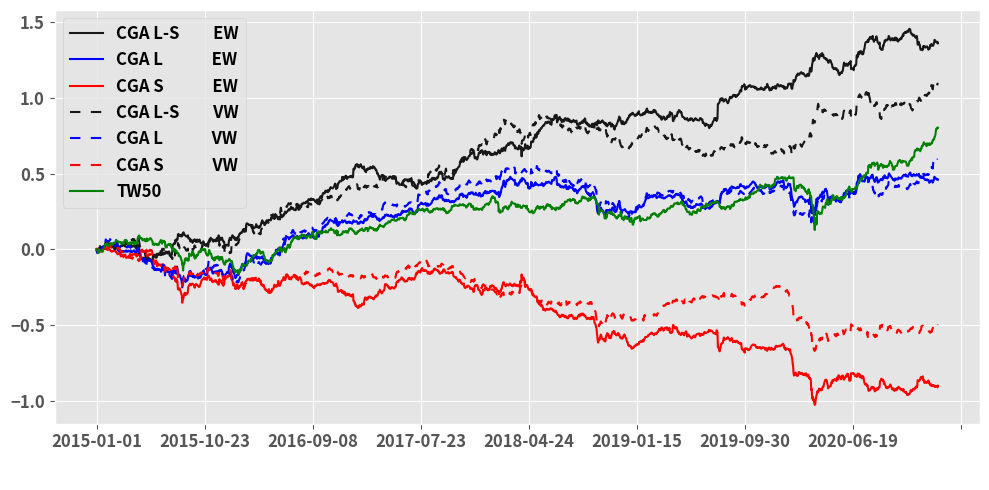
\includegraphics[width=1.1\textwidth]{images/CGA all.png}
\caption{CGA投組積效}
\end{figure}
於圖4.8繪製了利用CGA Predict所建構之投資組合「樣本外」累積對數報酬。黑線、藍線及紅線分別表示多空部位(Long-Short)、多頭部位(Long)及空頭部位(Short)之投資組合。實線及虛線則分別表示等權重(Equal-Weighted)及市值權重(Value-Weighted)兩種不同交易方式之投資組合績效。綠色實線表示買進並持有臺灣 50 (TW50)之報酬。根據上圖我們有以下三點結論,第一,我們可以看到在等權重以及市值權重中空頭部位之績效皆優於多頭部位之績效,我們做出以下之解釋:因為本研究只要研究台灣股市之市場,而台灣股市是一個以散戶為主之市場,而散戶交易人對於負面新聞較為敏感,若出現不利於所持有股票之新聞,較傾向受情緒左右而賣出部位,也顯示了散戶不理性之心態。第二,等權重投組之績效優於市值權重投組之績效,此結果顯示了在不考慮其他條件時,透過新聞文章所量化之情緒分數能較好的預測小型股票之報酬,我們針對此結果有以下解釋(1)投資者對於小型股票關注度較低且流動性不足等因素,因此新聞反應速度較慢。(2)小型股票之基本面相較於大公司之不確定性較為強烈,因此需要更多時間分析其新聞資訊。(3)大型股票受較多人研究與關注,所以其股價較不受新聞情緒因子所影響。第三,使用CGA Predict所建構之交易策略,於等權重多空部位投資組合以及市值權重多空部位投資組合,皆優於買進並持有臺灣50。

我們也檢驗了本研究所建構出新聞情緒因子是否會被Fama, French(1993)所提出之三因子以及Fama, French(2015)所提出之五因子解釋,根據表4.7可以發現,在所有三因子與五因子檢驗中之$R^{2}$皆小於$\alpha = 0.05$,亦即解釋能力皆為不顯著。
\begin{table}[H]
\begin{center}
\begin{tabular}[c]{cccm{1cm}<{\centering}m{1cm}<{\centering}m{1cm}<{\centering}m{1cm}<{\centering}m{1cm}<{\centering}m{1cm}<{\centering}}
\toprule
交易策略 & 夏普值  & 平均報酬 & FF3 &  & FF5 &  & FF5 + MOM & \\

Strategy & Sharpe Ratio & Average Return & $\alpha$ &  $R^{2}$  & $\alpha$ &  $R^{2}$ & $\alpha$ &  $R^{2}$ \\
\hline
CGA EW L-S & 1.18 & 6.97 & 7 & 0.6 & 7 & 0.7 & 7 & 0.7 \\
CGA EW L & 0.45 & 2.36 & 1 & 0.2 & 1 & 0.2 & 1 & 0.3\\
CGA EW S & 0.83 & 4.61 & 6 & 0.7 & 6 & 0.8 & 6 & 0.8\\
CGA VW L-S & 0.92 & 5.59 & 5 & 0.2 & 4 & 0.2 & 5 & 0.2\\
CGA VW L & 0.55 & 3.05 & 1 & 0.2 & 1 & 0.3 & 0.95 & 0.3\\
CGA VW S & 0.49 & 2.54 & 3 & 0.3 & 3 & 0.3 & 4 & 0.3\\
\bottomrule
\end{tabular}
\end{center}
\caption{三因子/五因子檢驗結果與CGA投資組合表現}
\label{Tab 4.7}
\end{table}
\footnotetext[1]{$R^{2}$單位:\%}
\subsection{新聞與價格延遲之關係與反應速度}
參考 Ke, Kelly, and Xiu (2019) 與 Fan, Xue, and Zhou (2021)近一步比較股票價格與新聞發佈時間之領先滯後關係。於訓練樣本中使用第T天所發佈之新聞對應至第T天之股票報酬訓練模型後分析樣本外第T天之新聞情緒與 T-1 天股票報酬 (第 T-1 天開盤至第 T 天開盤)、第 T 天股票報酬以及第 T+1 天股票報酬之間的關係,以 Day +1 ,Day -1 及 Day 0 三種不同的策略進一步的分析,探討台股市場中,投資人對於新聞消息之反應是否具有差異性,以及投資人是否有可能在新聞正式發佈以前便已經掌握未發布之新聞消息。
\begin{figure}[htbp]
\centering
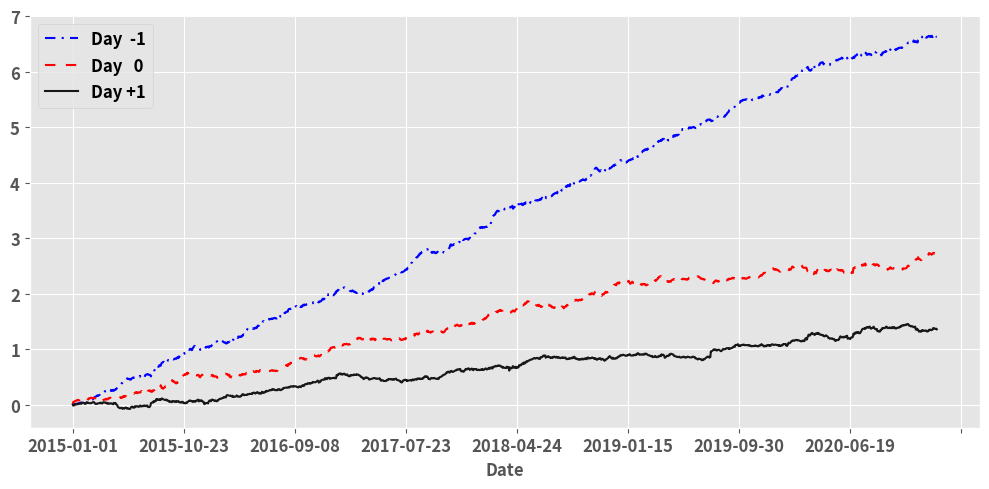
\includegraphics[width=1.1\textwidth]{images/speed0.png}
\caption{新聞情緒與價格延遲之關係}
\end{figure}

\newpage

在本小節我們比較了股票價格與新文發佈時間的關係,圖4.9分析了「樣本外」第 T 天新聞情緒與 T-1 天股票報酬、第 T 天股票報酬及第 T+1 天股票報酬之間的關係。Day -1 (藍色虛線) 為新聞情緒與新聞發佈前一天股票報酬之間的關係,而臺股於Day-1反應劇烈,顯示有部分報酬已透過內線反應至股價當中,意即市場上某些投資在新聞發布前便已知曉信息。Day 0 (紅色虛線)則為新聞情緒與發佈當天股票報酬之間的關係,可以發現大部分新聞訊息皆於新聞發布前後反應至股價當中,但是以上兩種策略為無法執行之交易策略,其所獲得之報酬為新聞發佈前之投資報酬,投資人於實盤交易之中無法於此二時段進行交易。

Day +1 (黑色實線)為新聞情緒與發佈隔天股票報酬之間之關係,為可行之交易策略,顯示了新聞情緒的延遲程度,該策略量化新聞情緒反應至股價中之「延遲程度」,可以看到 Day +1 策略仍可以帶來超額報酬,此結果顯示利用情緒因子所建構之投資組合仍然可以帶來超額報酬。


\subsection{異質性分析}
驗證領先滯後關係後本研究欲更深入針對不同類型股票之新聞反應時間進行異質性分析 (Heterogeneity Analysis),目的在於了解不同類型新聞之價格反應情形,欲使用市值與波動度兩個變數。使用市值之原因在於,因市值較大的公司代表著投資人將較多的資產分配於該公司股票,並且投資者容易將更多的注意力專注於大公司新聞 (Wilson (1975)、Veldkamp (2006))。因此基於每個時期台股上市公司市值中位數將股票分為大公司及小公司,並根據大小公司繪製每日平均報酬進行情緒訊息反應之比較分析,驗證投資者注意力之多寡是否影響相關新聞消息之反應。

再者使用波動度之原因在於,波動度係為套利交易之極限,在其他條件皆相同的情況下,股票波動度越高代表股票報酬的不確定性就越大。隨著更多的不確定性下,及可能使擁有越豐富資訊之投資者能獲得更高的報酬。然而,更多的不確定性也可能使該新聞之訊息較較難以被解釋,新聞所包含的情緒反應至股價之速度也較為緩慢。為驗證此現象也預計基於每個時期台股上市公司波動度中位數將股票分為高波動公司及低波動公司,並同樣根據高低波動公司繪製每日平均報酬進行比較分析。

\newpage

\begin{figure}[htbp]
\centering
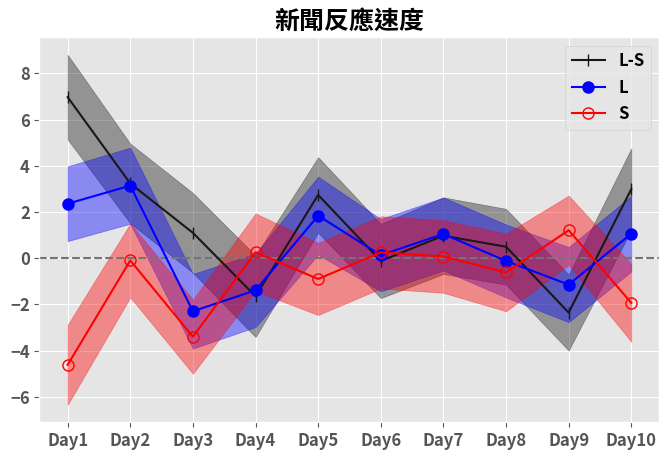
\includegraphics[width=1.1\textwidth]{images/speed1.png}
\caption{新聞反應速度}
\end{figure}

圖4.10繪製了用新聞情緒分數所建構之投資策略在新聞發佈後 1 至 10 日持有一日之每日平均報酬。如 Day 4 表示於新聞發佈後四日進行情緒分數交易策略之平均報酬(Average Returns)。陰影部分則為每日平均報酬之 95\%信賴區間。

本小節將進一步分析在延遲閱讀新聞下,進行情緒分數交易策略,則新聞情緒延遲反應之情形。圖4.10中繪製多空部位投資組合(Long-Short)以及多頭部位(Long)及空頭部位(Short)投資組合,圖中可發現對於多空策略,新聞情緒訊息於 Day+3時已經完全反應至股價當中。與美股市場不同的是,根據 Ke, et al. (2019) 研究顯示,美股新聞情緒訊息可以延續至Day+4始能反應完畢,顯示臺灣新聞情緒訊息大多於新聞發佈日或發佈前一天便提早反應至股價當中。

\newpage

\begin{figure}[htbp]
\centering
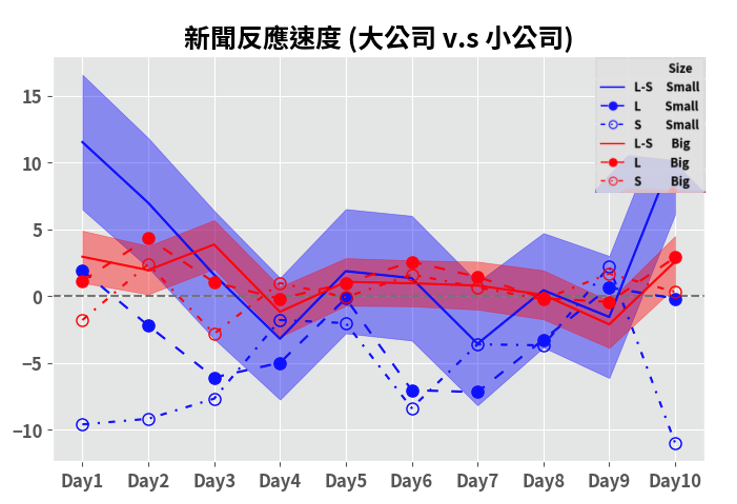
\includegraphics[width=1.1\textwidth]{images/speed2.png}
\caption{新聞反應速度(大公司 v.s 小公司)}
\end{figure}
圖4.11根據公司市值區分大公司及小公司繪製每日平均報酬(Average Returns)。區別大小公司之依據為利用每個時期台股上市公司市值中位數進行劃分。圖4.11中可發現小公司多頭部位在Day +1皆反應完畢,顯示了即便小公司出現正面新聞,投資者仍然較不傾向購入小公司之股票。小公司空頭反應至Day +4,顯示一旦小公司出現負面新聞,投資者傾向積極賣出小公司之股票,顯示了投資者之恐慌心理。大公司空頭於Day +1即反應完畢,顯示負面新聞較不影響投資人對於大公司股票持有之態度。

\newpage

\begin{figure}[htbp]
\centering
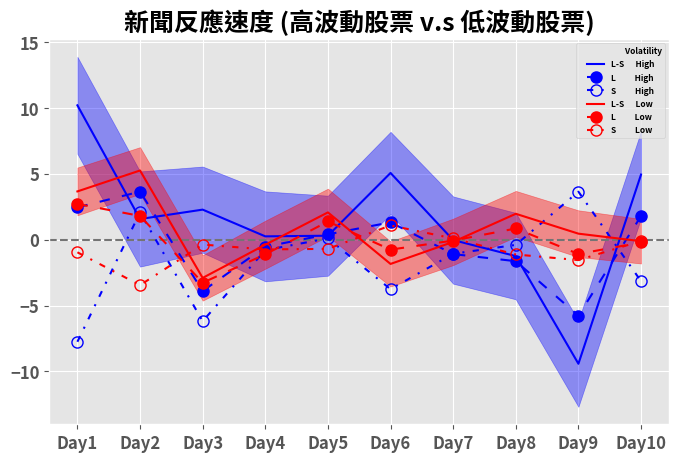
\includegraphics[width=1.1\textwidth]{images/speed3.png}
\caption{新聞反應速度(高波動 v.s 低波動)}
\end{figure}
圖4.12根據股票波動度區分高波動及低波動股票繪製每日平均報酬(Average Returns)。區別高低波動度股票之依據為每時期台股上市公司股票波動度中位數進行劃分。圖4.12可以發現,波動度越高,股票報酬之不確定性就越大,而隨著更多不確定性的產生,擁有更多資訊之投資者即可能獲得較高之報酬。然而,更多的不確定性代表該新聞訊息較難以被解釋,因此,新聞所包含的情緒訊息反應至股價的速度也較為緩慢,可以看到高波動公司需要三天才能將情緒完全反應至股價中。













